\section{Fault Modeling with Safety Annex}
\label{sec:fault_modeling}

%To align with the following paragraph from the Intro section
%In this paper we describe the \emph{Safety Annex} for the system engineering language AADL (Architecture Analysis and Design Language), a SAE Standard modeling language for Model-Based Systems Engineering (MBSE)~\cite{AADL_Standard}. 

\begin{comment}
%\subsection{Features Needed for Fault Modeling}
It is assumed that an AADL model of the nominal system specifies the hardware, software, and mechanical components of the system and their interconnections. This model is annotated with behavioral contracts using the AGREE annex~\cite{NFM2012:CoGaMiWhLaLu}. The nominal model behavioral requirements are verified using inductive model checking through AGREE~\cite{2017arXiv171201222G}. At this point, the fault modelling can commence. 

When conducting the safety assessment and examining the individual subcomponents of a system, the faults and failure modes must be determined. A fault is the manifestation of an error that may lead to failure in a given component~\cite{SAE:ARP4754A}. For example, a fault in a valve may be that it is stuck closed. If this fault is active, it may cause a failure to occur. If there is no command to provide outgoing pressure, then this active fault will not cause a failure of the component to perform as intended. On the other hand, if there is such a command to provide pressure, this fault will cause failure of the valve component. The failure mode in this case is that there is a command to provide outgoing pressure, but an active fault on the valve causes it to be stuck closed. We use {\em fault} as the generic modeling keyword throughout the AADL model hierarchy and follow the definitions of these terms (error, failure, fault) throughout this description.

Many of these modes can be determined through domain knowledge and other modes are specified through the manufacturer of a given mechanical or digital component. Once the faults and failure modes are determined, the safety engineer must determine the consequence of this component failure on connected components, components that are physically located nearby, and on the system as a whole. Given that many safety critical systems are quite complex, this propagation process can be error prone and time consuming.

In the following subsections, we walk through examples of component failure modes to illustrate how a safety engineer can use the Safety Annex to model these modes and see how an active fault may or may not cause failure of a component.
\end{comment}


%When conducting the safety assessment and examining the individual subcomponents of a system, the faults and failure modes must be determined. A fault is the manifestation of an error that may lead to failure in a given component~\cite{SAE:ARP4754A}. For example, a fault in a valve may be that it is stuck closed. If this fault is active, it may cause a failure to occur. If there is no command to provide outgoing pressure, then this active fault will not cause a failure of the component to perform as intended. On the other hand, if there is such a command to provide pressure, this fault will cause failure of the valve component. The failure mode in this case is that there is a command to provide outgoing pressure, but an active fault on the valve causes it to be stuck closed. We use {\em fault} as the generic modeling keyword throughout the AADL model hierarchy and follow the definitions of these terms (error, failure, fault) throughout this description.

%Many of these modes can be determined through domain knowledge and other modes are specified through the manufacturer of a given mechanical or digital component. Once the faults and failure modes are determined, the safety engineer must determine the consequence of this component failure on connected components, components that are physically located nearby, and on the system as a whole. Given that many safety critical systems are quite complex, this propagation process can be error prone and time consuming.

In the following subsections, we walk through examples of component failure modes to illustrate how a safety engineer can use the Safety Annex to model these modes and see how an active fault may or may not cause failure of a component.

%In the AADL system model and the AGREE behavioral model, we have the component structures and behaviors (properties) defined for the system subcomponents. Assuming that the nominal model holds (in the absence of errors, the system behavior is correct), it is of interest to see how the manifestation of errors impacts the overall system functionality. To determine this information, a safety engineer must determine what possible errors could be present in the given components of the system and if the manifestation of these errors will cause a systems functionality to be erroneous. Many of these component errors originate in software and when these errors manifest in real life, they are propagated implicitly through the system. For example, when a valve is stuck closed the effects of this component failure can be seen through the behavioral contracts and need not be explicitly modeled. But this does not cover all possible failure types. As an example, assume there are co-located pipes and one bursts. Given the nature of the failure, this could affect the behavior of the co-located pipe and thus must be explicitly propagated. In the system model, there are no connections between these components, only in the physical world are they related. For this reason, a safety analyst must be able to define explicit propagation as well as implicit.  

%In the following subsections, we describe the modeling process for these failure modes using the WBS as a reference model. 

 \subsection{The Wheel Brake System Example}
\label{sec:case_study} 

%\subsubsection{Wheel Brake System}
In order to demonstrate the fault modeling capabilities of the Safety Annex in Section~\ref{sec:fault_modeling} and provide examples of how to use the Safety Annex to perform fault modelling and analysis, we describe a model of a Wheel Brake System (WBS) of an aircraft. 

The Wheel Brake System (WBS) described in AIR6110~\cite{AIR6110} is a well-known example that has been used as a case study for safety analysis, formal verification, and contract based design~\cite{DBLP:conf/cav/BozzanoCPJKPRT15, 10.1007/978-3-319-11936-6-7, CAV2015:BoCiGrMa, Joshi05:SafeComp}. The preliminary work for the safety annex used a simplified model of the WBS~\cite{Stewart17:IMBSA}. In order to demonstrate a complex fault modeling process, we constructed a functionally and structurally equivalent AADL version of one of the most complex WBS NuSMV/xSAP models (arch4wbs) described in~\cite{DBLP:conf/cav/BozzanoCPJKPRT15}.    

\begin{figure}[h!]
	\centering
	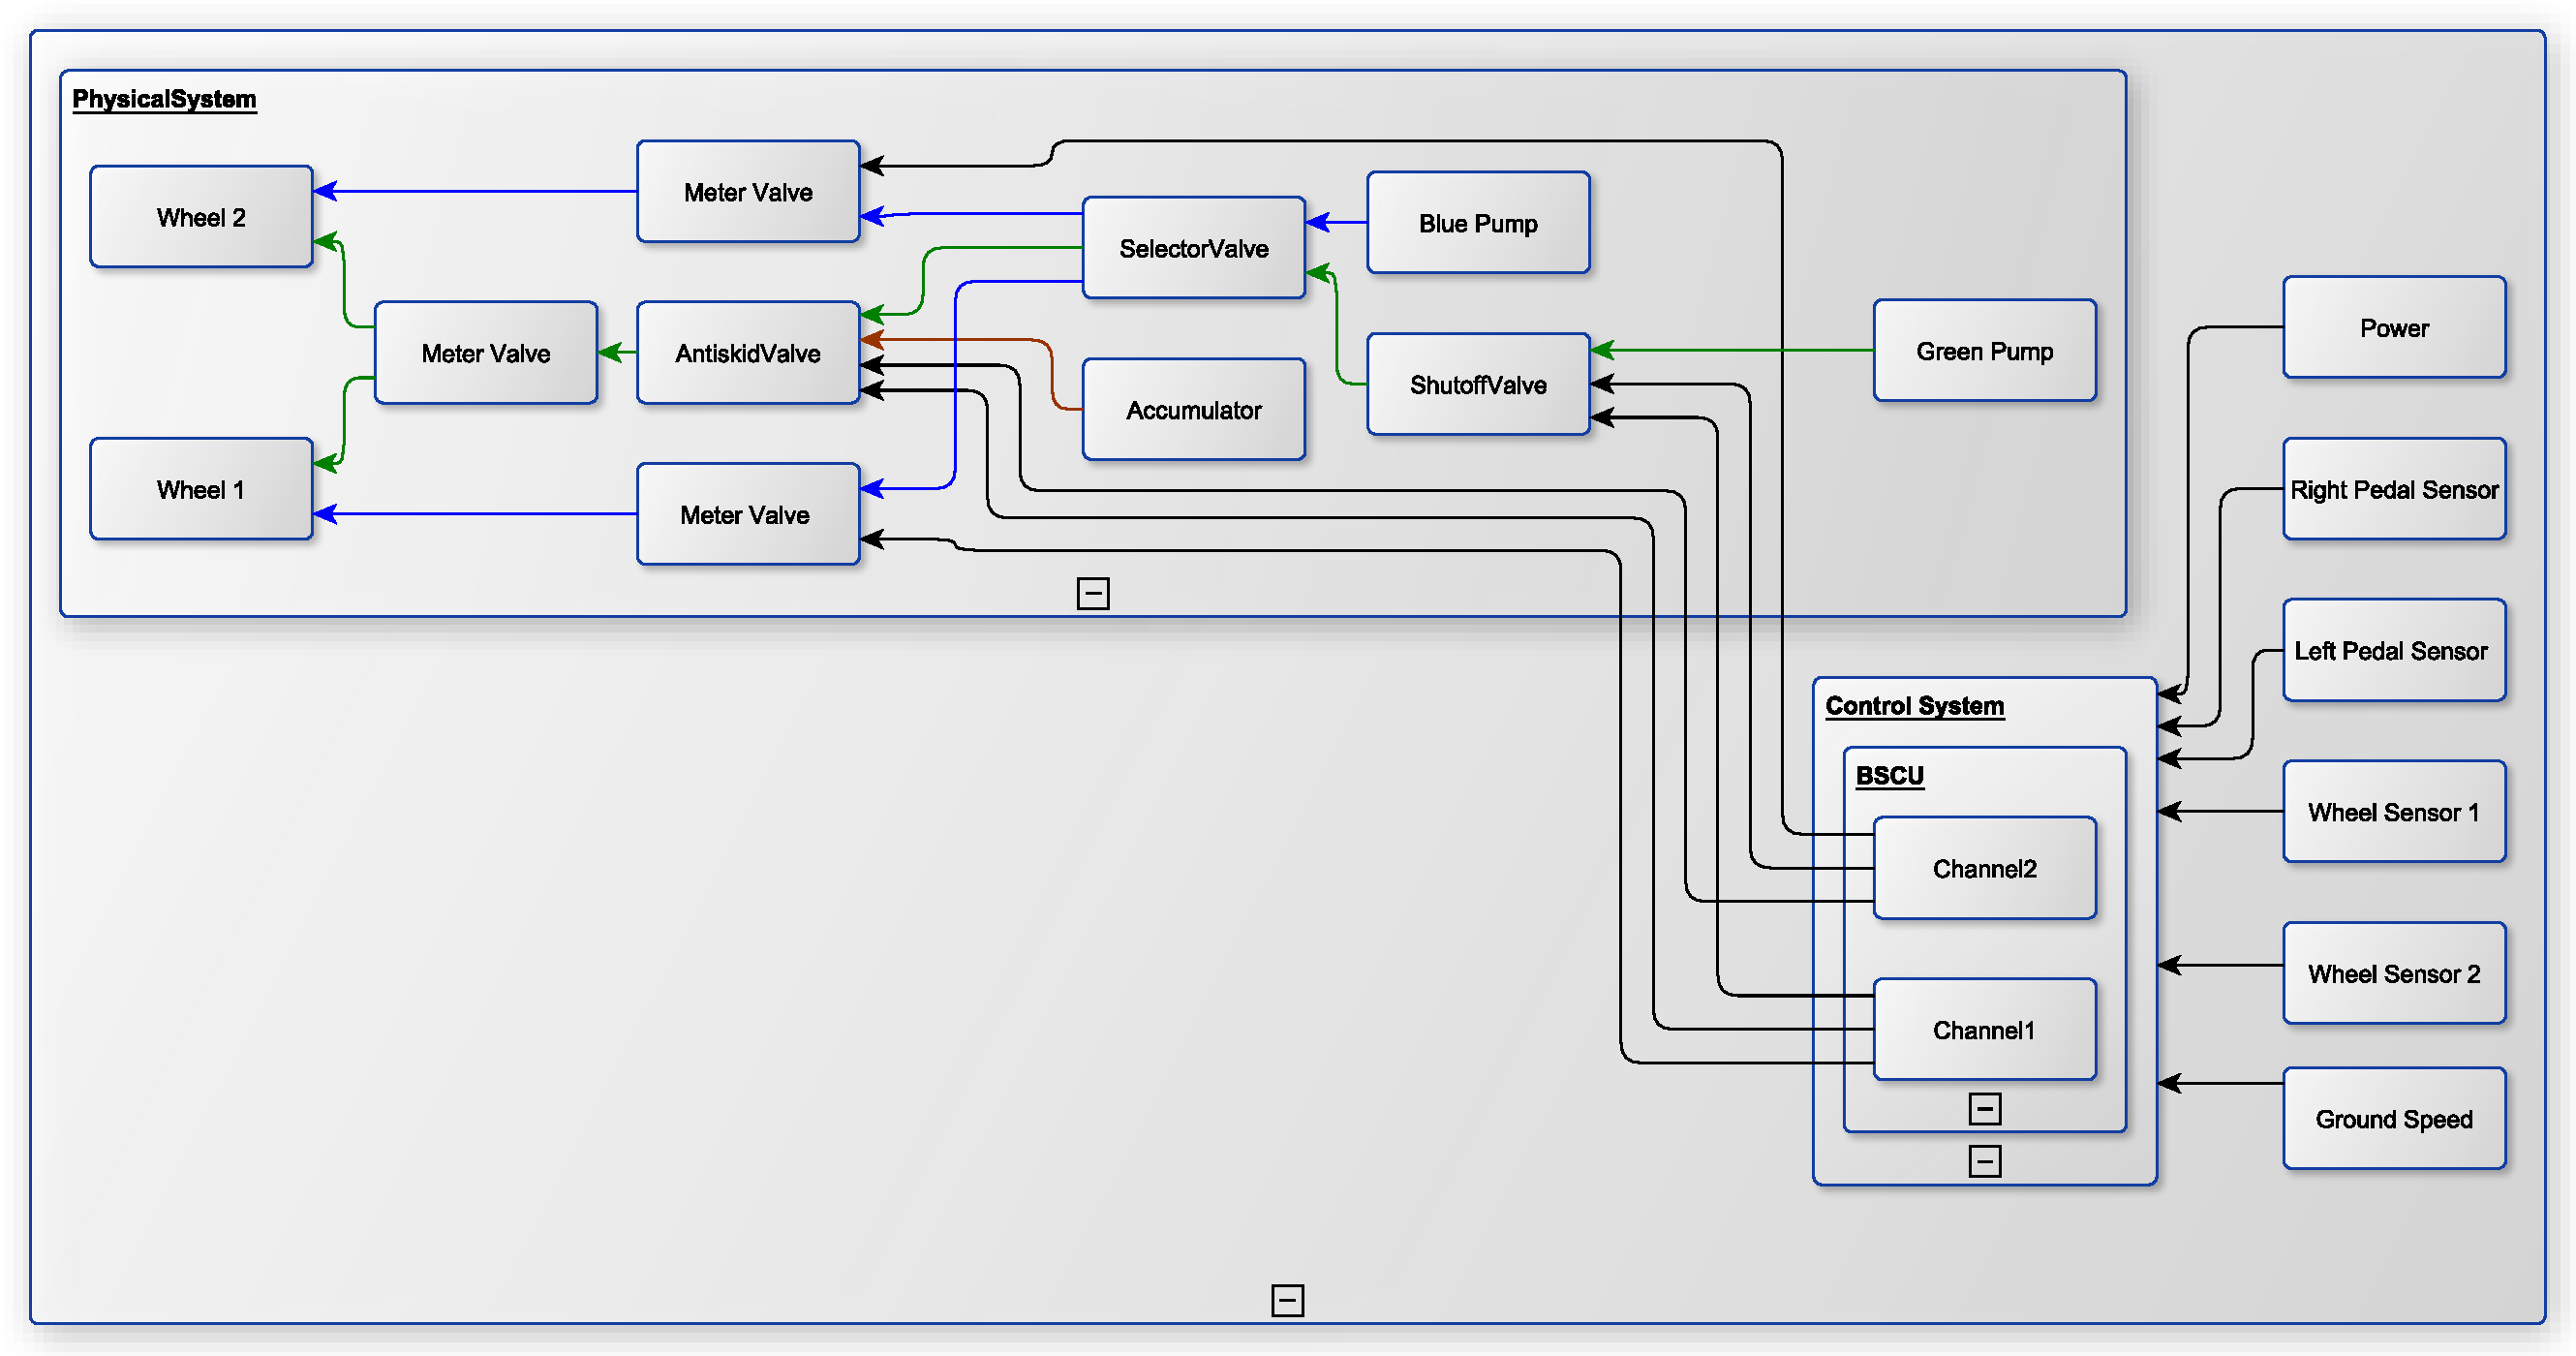
\includegraphics[trim=0 9 0 5,clip,width=\textwidth]{images/wbs_arch.pdf}
	\caption{Wheel Brake System}
	\label{fig:wbs}
\end{figure} 

%\subsubsection{WBS Architecture Description}
The WBS is composed of two main parts: the control system and the physical system. The control system electronically controls the physical system and contains a redundant channel of the Braking System Control Unit (BSCU) in case of failure. It also commands antiskid braking in case of skidding on the ground. The physical system consists of the hydraulic circuits running from hydraulic pumps to wheel brakes as well as valves that control the hydraulic fluid flow. This is what provides braking force to each of the 8 wheels of the aircraft. The wheels are all mechanically braked in pairs (one pair per landing gear). For simplicity's sake, Figure~\ref{fig:wbs} displays only two of the 8 wheels. 

There are three operating modes in the WBS model. In \textit{normal} mode, the system uses the \textit{green} hydraulic circuit. The normal system is composed of the green hydraulic pump and one meter valve per each of the 8 wheels. Each of the meter valves are controlled through electronic commands coming from the active channel of the BSCU. These signals provide braking and antiskid commands for each wheel. The braking command is determined through a sensor on the pilot pedal position and is labeled as \textit{Left/Right Pedal Sensor} in Figure~\ref{fig:wbs} and the antiskid command is determined by the \textit{Wheel Sensors}. 

In \textit{alternate} mode, the system uses the \textit{blue} hydraulic circuit. The alternate system is composed of the blue hydraulic pump, four meter valves, and four antiskid shutoff valves: one for each landing gear. The meter valves are mechanically commanded through the pilot pedal corresponding to each landing gear. If the system detects lack of pressure in the green circuit, the BSCU channel commands the selector valve to switch to the blue circuit. %This switch can occur, for example, if there is a lack of pressure from the green hydraulic pump, the green hydraulic pump circuit fails, or pressure is cut off by a shutoff valve. 
If the BSCU channel becomes invalid, the shutoff valve closes and we move into alternate mode. Once this system switches into alternate mode, it does not return to normal operation mode.

The last mode of operation of the WBS is the \textit{emergency} mode. This mode is entered if the blue hydraulic pump fails. The accumulator pump has a reserve of pressurized hydraulic fluid and will supply this to the blue circuit in emergency mode.

%To get an idea of the size of this model, the system model contains 30 different kinds of components, 169 component instances, and a model depth of 5 hierarchical levels. 

The model contains 30 different kinds of components, 169 component instances, a model depth of 5 hierarchical levels.  The model includes one top-level assumption and  11 top-level system properties, with 113 guarantees allocated to subsystems.  There are a total of 33 different fault types and 141 fault instances within the model.  The large number of fault instances is due to the redundancy in the system design and its replication to control 8 wheels.

The behavioral model is encoded using the AGREE annex and the behavior is based on descriptions found in AIR6110. The top level system properties are given by the requirements and safety objectives given in AIR6110. All of the subcomponent contracts support these system safety objectives through the use of assumptions on component input and guarantees on the output.

An example property is to ensure no inadvertent braking of each of the 8 wheels. This is based on one of the failure conditions described in AIR6110 is \textit{Inadvertent wheel braking of all wheels during takeoff roll after V1 shall be less than 1E-9 per takeoff}. 

This property can be broken down as follows. In order for no inadvertent braking to occur, there needs to be a series of behaviors that occur in the system simultaneously. The system is provided with both power and hydraulic pressure and the pilot has not pressed the brake pedal. At the same time, the plane is not stopped, there is braking force at the wheel, and the wheel is rolling. When all of these things happen together, this is inadvertant braking. Naturally, the safety property states this as all of these things do \textit{not} occur together. Given a model of this size, it can be complicated to determine the combinations of component errors that could occur in order to lead to a functional failure.


\subsection{Fault Modeling}
%To align with the following intro section
%The Safety Annex allows an analyst to model the failure modes of components and then ``weave'' these failure modes together with the original models developed as part of MBSE. 
%The safety analyst can then leverage the merged behavioral models to propagate failures through the system to investigate their effect on the safety requirements (implicit failure propagation). 

When using the Safety Annex to model behavioral failure propagation, a \textit{fault} is attached to a component, which when active will change the output of said component. This faulty value on the output may or may not violate the contracts of the component and it may or may not violate the assumptions of the destination component. These details are seen through the output of the model checker when the safety analysis is run on the fault model. Examples of such faults include valves being stuck open or closed, output of a software component being nondeterministic, or power being cut off. These component types range from mechanical to digital, but for this section we focus on a digital component in the WBS, a sensor on the pedal component. 

The purpose of the safety analysis process is to guarantee that certain top level safety properties of the system hold with certain reliability in the presence of faults. 

%One of the failure conditions described in AIR6110 is \textit{Inadvertent wheel braking of all wheels during takeoff roll after V1 shall be less than 1E-9 per takeoff}. Due to the catastrophic classification of this hazard, this is a property we chose for illustrative purposes. 

%This property can be broken down as follows. In order for no inadvertent braking to occur, there needs to be a series of behaviors that occur in the system simultaneously. The system is provided with both power and hydraulic pressure and the pilot has not pressed the brake pedal. At the same time, the plane is not stopped, there is braking force at the wheel, and the wheel is rolling. When all of these things happen together, this is inadvertant braking. Naturally, the safety property states this as all of these things do \textit{not} occur together. Given a model of this size, it can be complicated to determine the combinations of component errors that could occur in order to lead to a functional failure.

One of the components important to the property \textit{Inadvertant braking}, is the pedal. When the mechanical pedal is pressed, a sensor reads this information and passes an electronic signal to the BSCU which then proceeds in commanding hydraulic pressure to the wheels. 

\begin{figure}[h!]
	\hspace*{-2cm}
	\vspace{-0.4in} 
	\begin{center}
		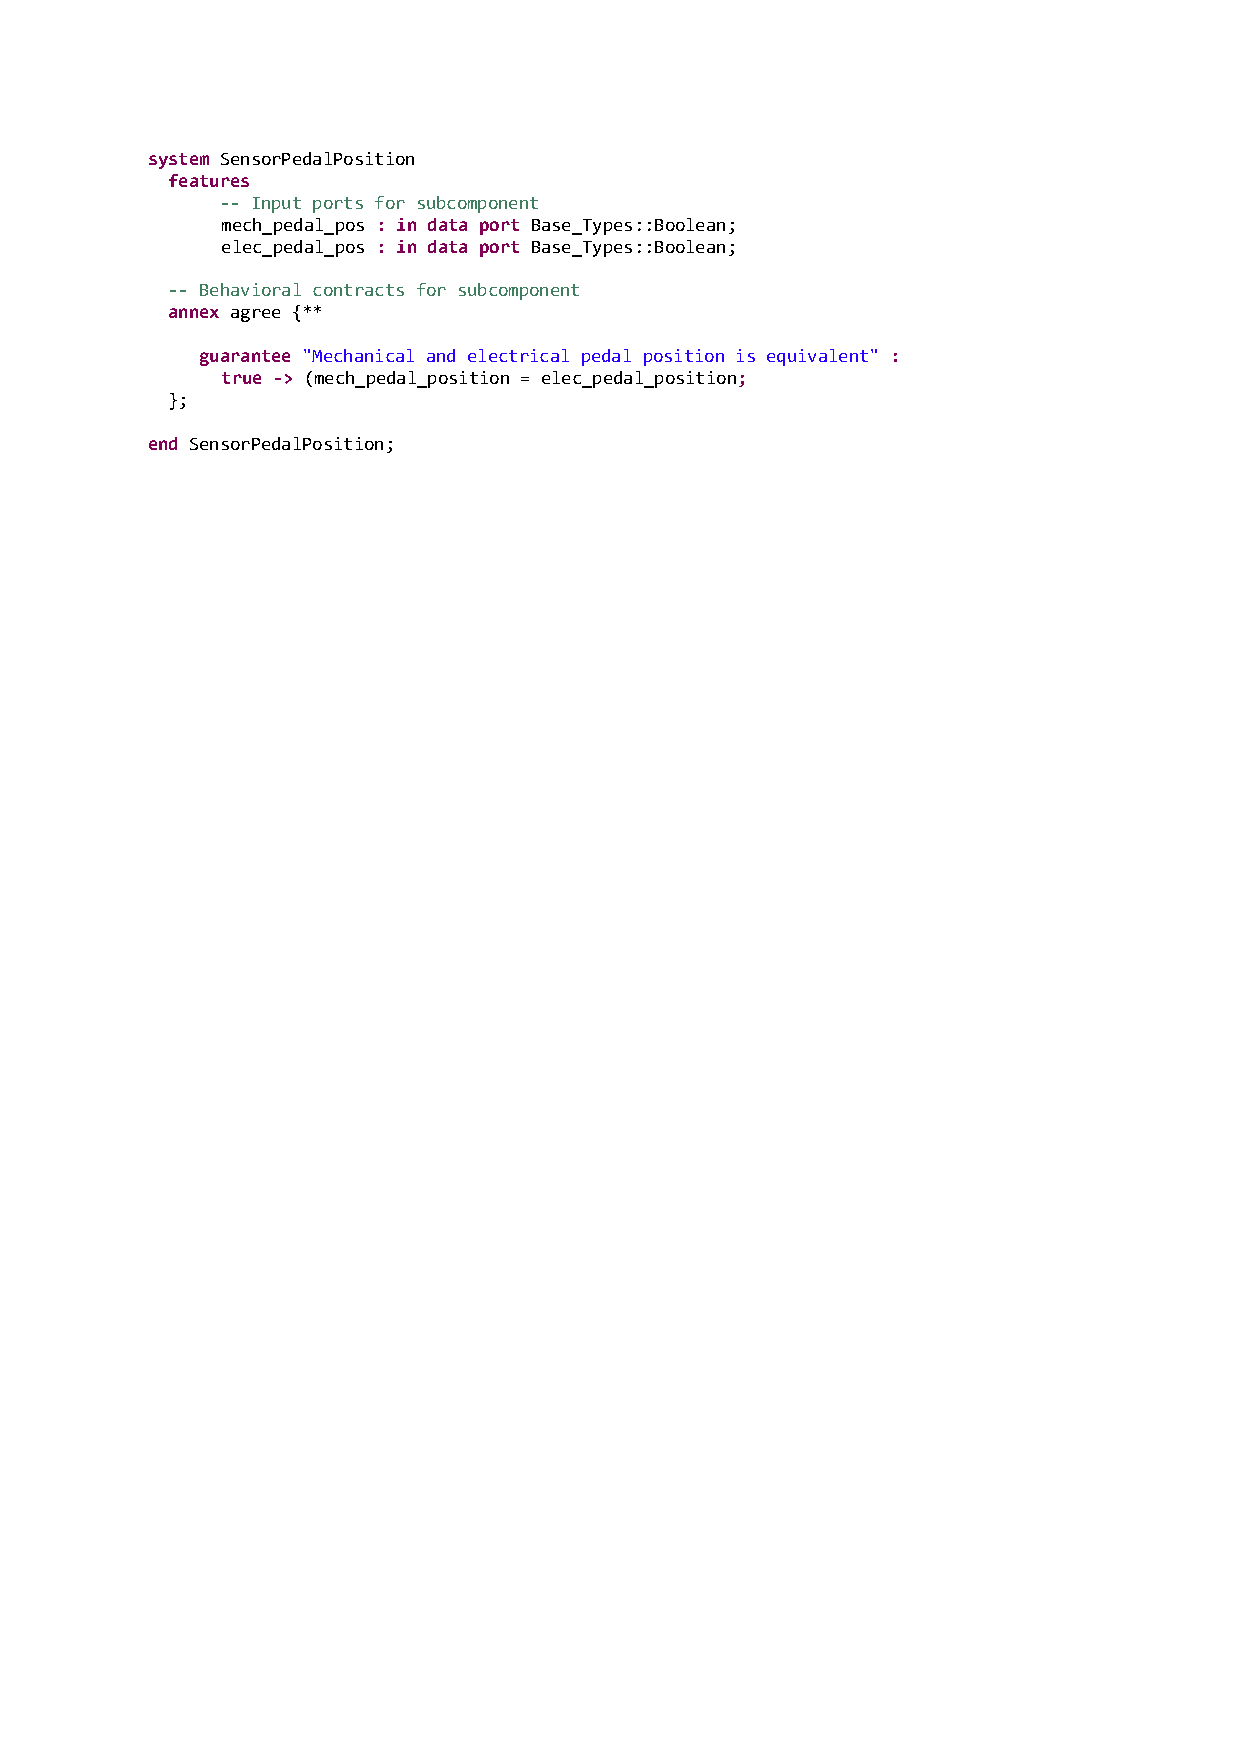
\includegraphics[trim=0 640 -10 70,clip,width=1.5\dimexpr\textwidth-2cm\relax]{images/system_sensor.pdf}
		\caption{An AADL System Type: The Pedal Sensor}
		\label{fig:sensor}
	\end{center}
	\vspace{-0.3in}
\end{figure}

In Figure~\ref{fig:sensor}, the AADL system component is shown with a contract on the output of this component. The sensor has only one input: the mechanical pedal position and one output: the electrical pedal position. The property that governs the behavior of the component is that the mechanical position should always equal the electronic position. This is an example of the nominal system model in AADL with behaviors defined in AGREE. 

\begin{figure}[h!]
	\hspace*{-2cm}
	%\vspace{-0.4in} 
	\begin{center}
		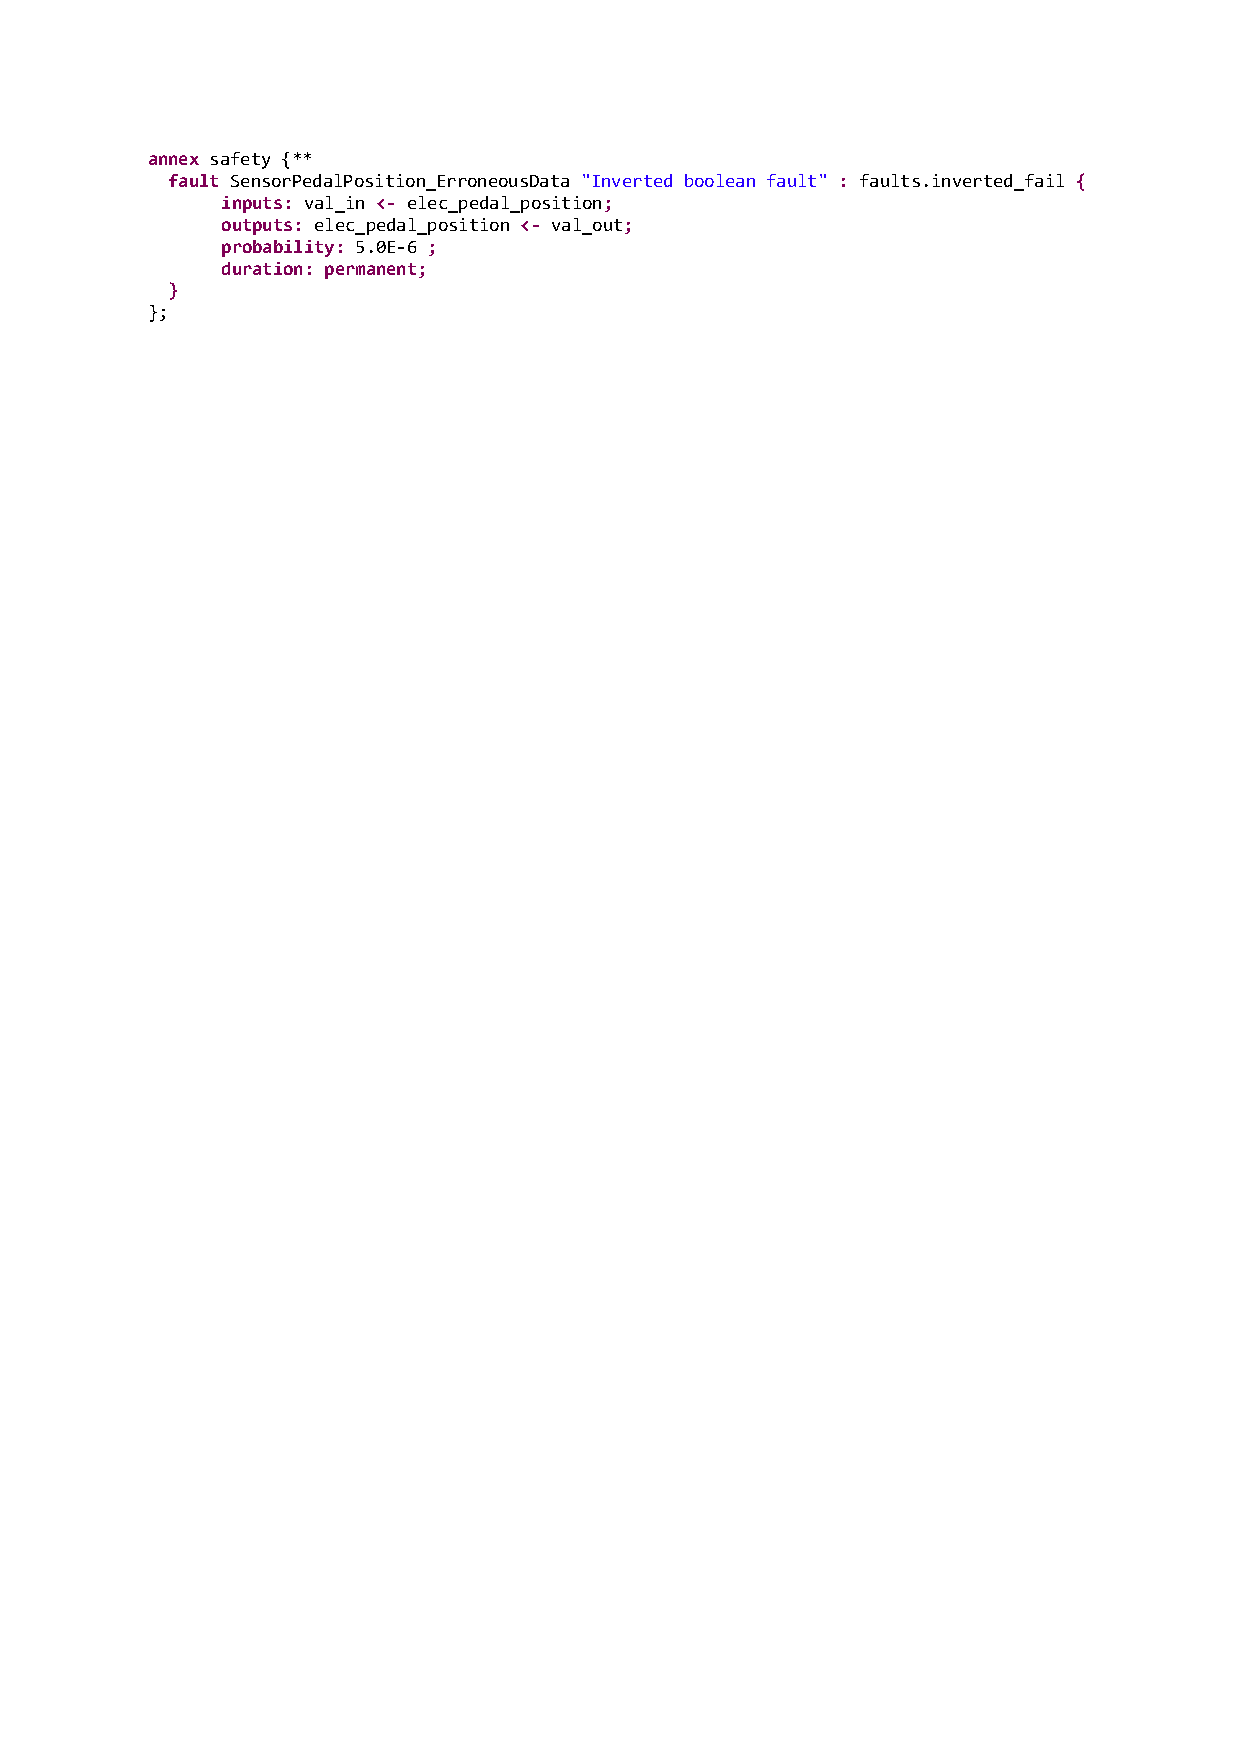
\includegraphics[trim=0 690 -10 70,clip,width=1.5\dimexpr\textwidth-2cm\relax]{images/safetyannex_sensorfault.pdf}
		\caption{The Safety Annex for the Pedal Sensor}
		\label{fig:sensorFault}
	\end{center}
	\vspace{-0.3in}
\end{figure}

This sensor has a known failure which can invert the signal read and pass along an incorrect value. This fault which causes this failure is triggered with probability $5.0e-6$. In Figure~\ref{fig:sensorFault}, the Safety Annex definition for this fault is shown. The faults are defined using a library of fault nodes (in this case, \textit{inverted\_fail}) and when the fault is triggered, the output of the component (\textit{elec\_pedal\_position}) is converted into its failure value (\textit{val\_out}). 

\subsection{Concept of Implicit Behavioral Propagation}

The AADL language has previously been extended to provide some fault modeling and analysis capabilities using its Error Model Annex, Version 2 (EMV2)~\cite{EMV2}.  EMV2 focuses on injection and propagation of discrete faults for generation of fault trees, rather than on analysis of system behavior in the presence of faults. 
To illustrate some of the key differences between our approach and the EMV2 approach, Figure~\ref{fig:comparison_with_EMV2} shows a simplified WBS example. The code fragments in the figure extracted from EMV2, AGREE, and the Safety Annex do not represent the complete code.

\begin{figure}[t]
	\vspace{-0.19in}
	\centering
	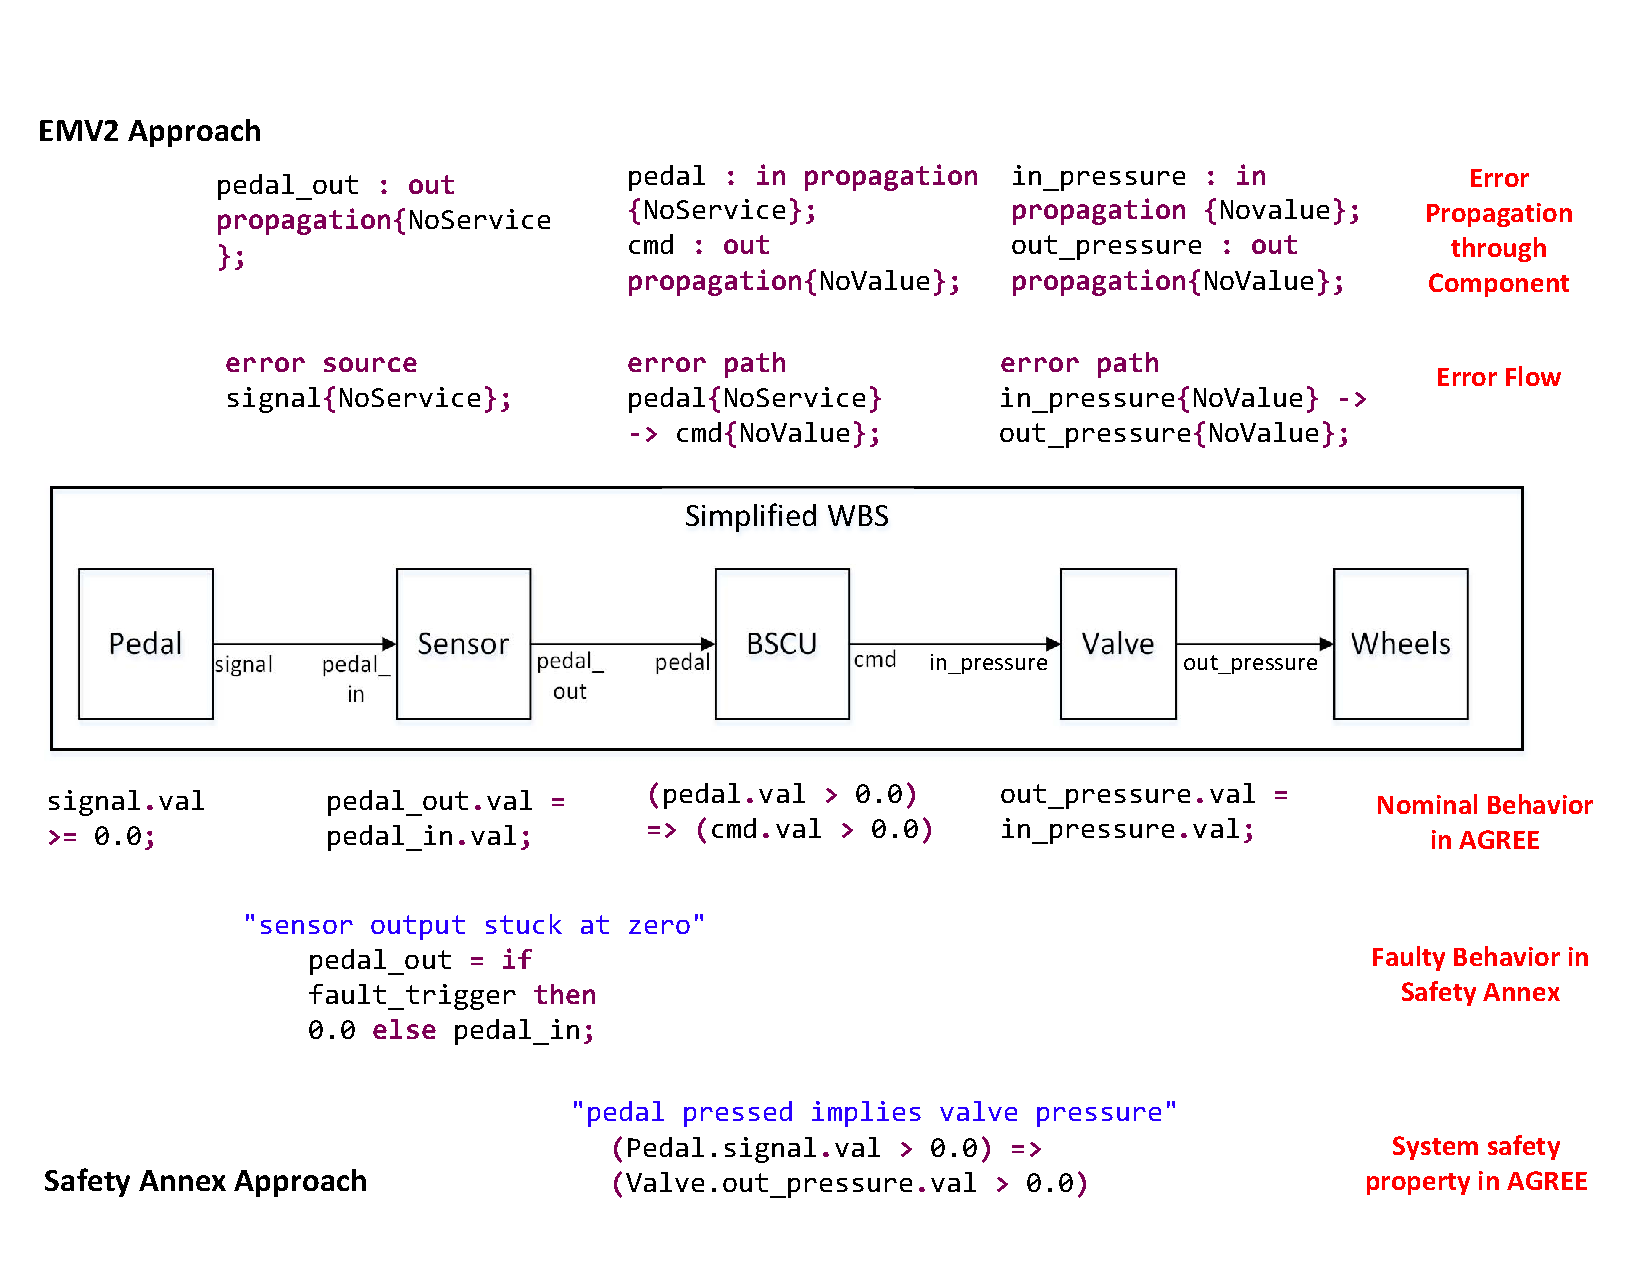
\includegraphics[trim=0 9 0 5,clip,width=\textwidth]{images/Comparison_with_EMV2.pdf}
	%\vspace{0.4in}
	\caption{Differences between Safety Annex and EMV2}
	\label{fig:comparison_with_EMV2}
\end{figure} 

In this simplified WBS system, the physical signal from the Pedal component in detected by the Sensor, and the pedal position value is passed to the Braking System Control Unit (BSCU) components.  The BSCU generates a pressure command to the Valve component which applies hydraulic brake pressure to the Wheels. In this example, we use the general term ``fault'' to denote all component errors, hardware failures, and system faults captured by both approaches.

In the EMV2 approach (top half of Figure~\ref{fig:comparison_with_EMV2}), all faults must be explicitly propagated through each component (by applying fault types on each of the output ports) in order for a component to have an impact on the rest of the system. In the example, the ``NoService'' fault is explicitly allowed by the EMV2 declarations to propagate through all of the components.  These fault types are essentially tokens that do not capture any analyzable behavior.  At the system level, analysis tools supporting the EMV2 annex can aggregate the fault flow and propagation information from different components to compose an overall fault flow diagram or fault tree.

In the Safety Annex approach (bottom half of Figure~\ref{fig:comparison_with_EMV2}), faults are captured as faulty behaviors that augment the system behavioral model in AGREE contracts.  When a fault is triggered, the output behavior of the Sensor component is modified, in this case resulting a ``stuck at zero'' error. The behavior of the BSCU receives a zero input and proceeds as if the pedal has not been pressed. This will cause the top level system contract to fail: {\em pedal pressed implies brake pressure output is positive}. No explicit fault propagation is necessary since the faulty behavior itself propagates through the system just as in the nominal system model. The effects of any triggered fault are manifested through analysis of the AGREE contracts. 


%Moved to the analysis section
%When this particular fault is active in the system, we can run the analysis to see how it propagates through the system. The classification of the top level safety property is catastrophic and carries a probability threshold of $1.0e-9$. Since the probability of this fault occurring on the sensor is higher than that of the top level property, it is of relevance. 

%Upon running the fault analysis in the toolset, a counterexample is provided for this top level property given the fault definition provided in Figure~\ref{fig:sensorFault}. Through the counterexample display we can trace the behavior of the system through the active faults as well as the violated contracts. The mechanical pedal is not pressed, but this failure causes the sensor subcomponent to report to the BSCU that it was pressed. The active BSCU channel uses this value in order to command braking, determine the validity of the channel and control the antiskid behavior of the aircraft. The BSCU carries on with its normal behavior assuming that the pedal was pressed and the state of the system is as follows: braking is not commanded and power is supplied throughout the system. The ground is moving, there is braking force at the wheels, and the wheel is rolling. Taken together this clearly disproves the top level contract that inadvertent braking at a given wheel does not occur. Thus the safety analyst of this system can recognize that some set of precautions such as redundancy are required for the pedal sensor component. 

\subsection{Explicit Failure Propagation} 
%To align with the following intro paragraph
%In addition, the annex allows modeling of explicit failure propagation that is not captured through the behavioral models, for example, the effect of a single electrical failure on multiple software components or the effect hardware failure (e.g., an explosion) on multiple behaviorally unrelated components. 

%As described in Section~\ref{subsec:comparison_with_EMV2}, explicit fault propagation is something that currently exists in EMV2 for AADL and the mode of fault analysis presented in this paper is behavioral fault propagation. But there is another set of possible failures in a system that are difficult to capture with the fault definitions previously discussed. 

Faults in hardware (HW) components can trigger behavioral faults in the software (SW) or system components that depend on them. For example, a CPU fault may trigger faulty behavior in the threads bound to that CPU. In addition, a fault in one HW component may trigger faults in other HW components located nearby, such as overheating, fire in the containment location, or a stray bullet. 

To better model HW dependent faults, a fault model element is introduced for HW components called a \textit{hardware} fault. Users are not required to specify behavioral effects for the HW faults, nor are data ports necessary on which to apply the fault definition. 

%Failures in hardware (HW) components can trigger behavioral faults in the software (SW) or system (SYS) components that depend on them.  For example, a CPU failure may trigger faulty behavior in threads bound to that CPU. In addition, a failure in one HW component may trigger failures in other HW components located nearby, such as cascading failure caused by a fire or water damage.

%Faults propagate in AGREE as part of a system’s nominal behavior. This means that any propagation in the HW portion of an AADL model would have to be artificially modeled using data ports and AGREE behaviors in SW. This is less than ideal as there may not be concrete behaviors associated with HW components. In other words, faulty behaviors mainly manifest themselves on the SW/SYS components that depend on the hardware components.

%To better model faults at the system level dependent on HW failures, we have introduced a new fault model element for HW components. In comparison to the basic fault statement introduced in the previous section, users are not specifying behavioral effects for the HW failures, nor data ports to apply the failure. 
An example of a model component fault declaration is shown below:
\begin{figure}[h!]
	\vspace{-0.2in}
	\begin{center}
		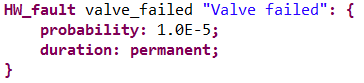
\includegraphics[width=.5\textwidth]{images/hw_fault.png}
	\end{center}
	\vspace{-0.4in}
\end{figure}

Users specify dependencies between the HW component faults and faults that are defined in other components, either HW or SW. The hardware fault then acts as a trigger for dependent faults. This allows a simple propagation from the faulty HW component to the SW components that rely on it, affecting the behavior on the outputs of the affected SW components.

The fault dependencies are typically specified in the system implementation where the system configuration that causes the dependencies becomes clear (e.g., binding between SW and HW components, co-location of HW components). This is because fault propagations are typically tied to the way components are connected or bound together; this information may not be available when faults are being specified for individual components. Having fault propagations specified outside of a component’s fault statements also makes it easier to reuse the component in different systems. 

An example of a fault dependency specification is shown below, showing that the valve{\_}failed fault at the shutoff subcomponent triggers the pressure{\_}fail{\_}blue fault at the selector subcomponent.
\begin{figure}[h!]
	\vspace{-0.2in}
	\begin{center}
		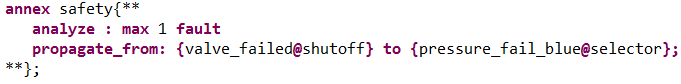
\includegraphics[width=.9\textwidth]{images/fault_propagation.png}
	\end{center}
	\vspace{-0.4in}
\end{figure}


\begin{comment}
%In complex systems, it can be difficult to determine the effects of HW faults on SW functions. By utilizing a simple propagation from the faulty HW component to the SW components that rely on it, the behavior and outputs of the affected SW functions can be realized. 

\begin{figure}[h!]
	\hspace*{-2cm}
	\vspace{-0.3in} 
	\begin{center}
		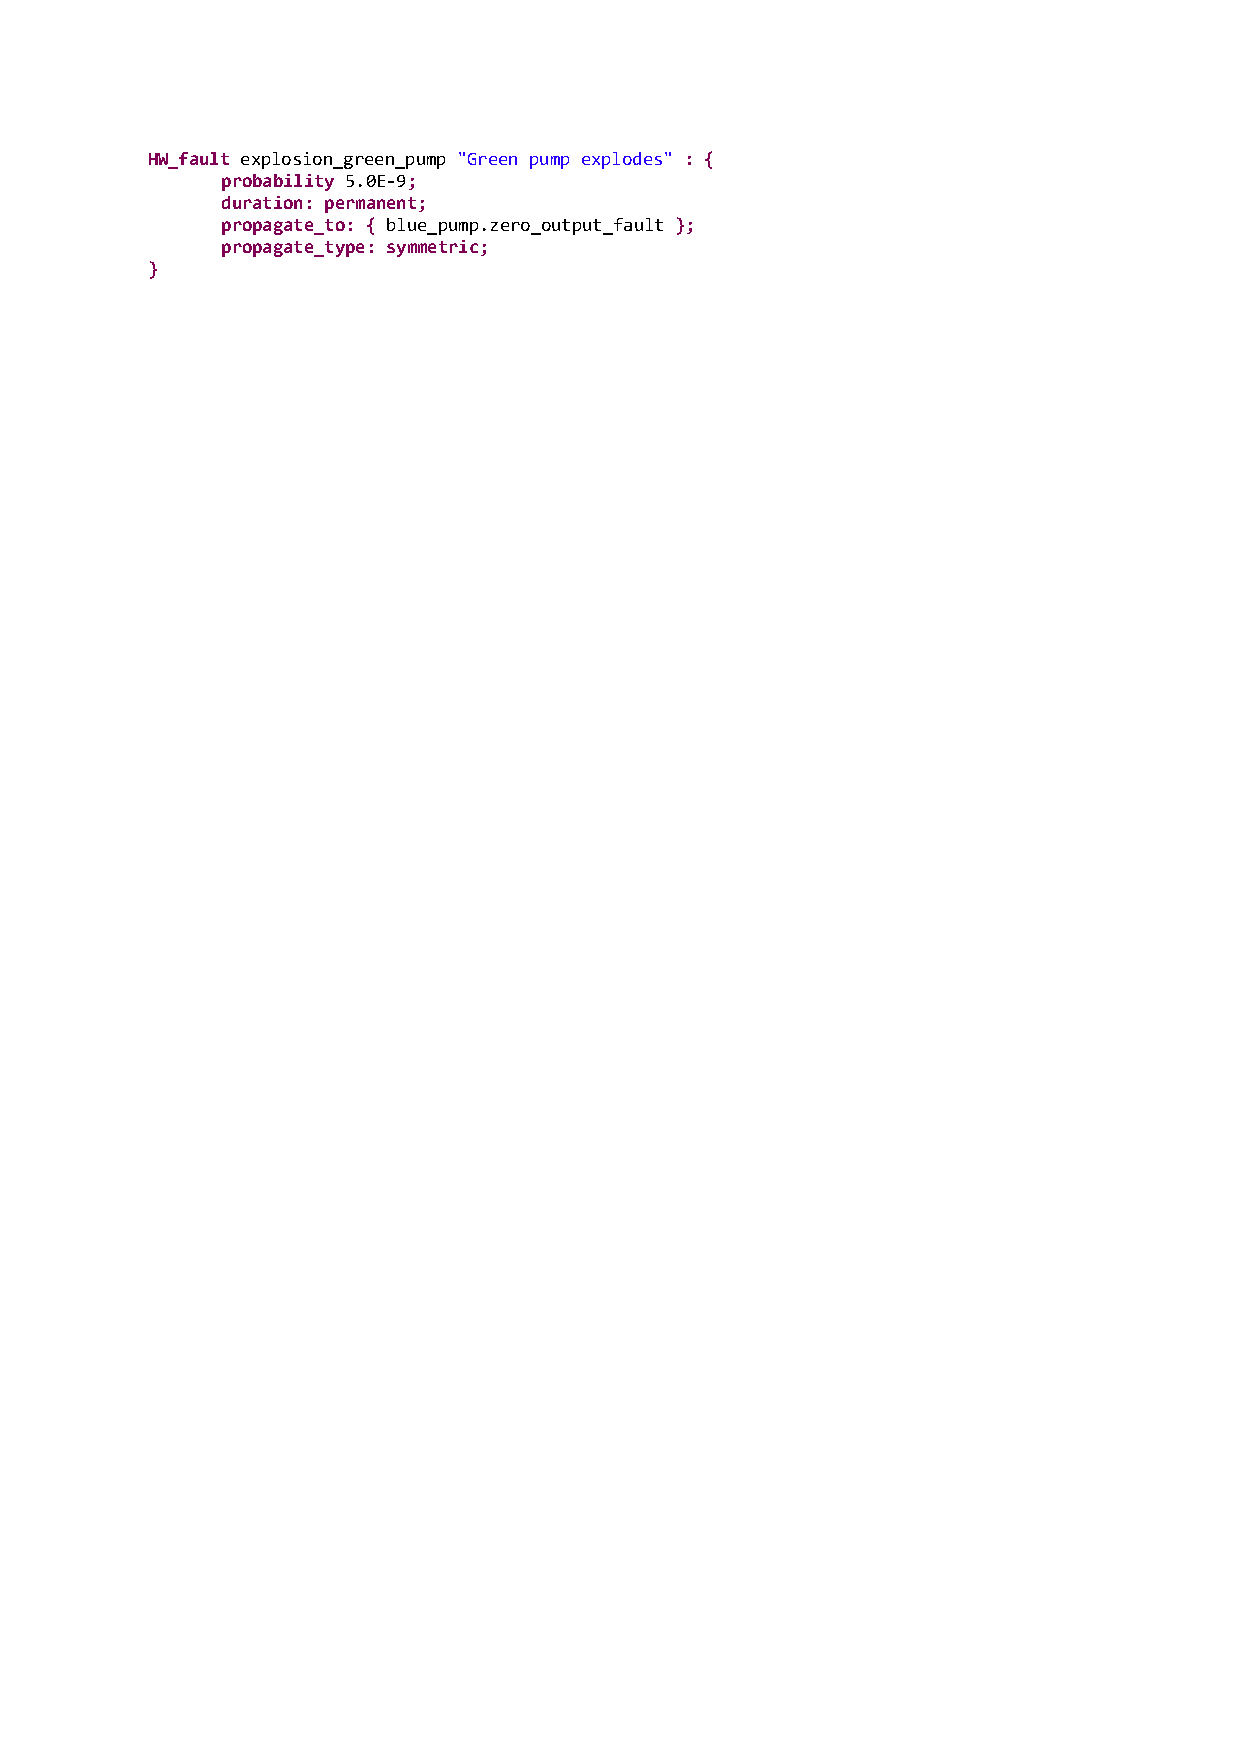
\includegraphics[trim=0 690 -10 70,clip,width=1.5\dimexpr\textwidth-2cm\relax]{images/hw_fault_green_pump.pdf}
		\caption{Hardware fault for the green pump}
		\label{fig:hwFault}
	\end{center}
	\vspace{-0.3in}
\end{figure}

As an example, we will look yet again at the WBS. Assume that both the green and blue hydraulic pumps are located in the same compartment in the aircraft. When an explosion took place in said compartment, the green (normal) hydraulic pump took the force of the explosion and when the green hydraulic pump exploded, the pump shrapnel flew into the blue (alternate) pump and it became from then on unoperable. 
%This particular aircraft was in flight when the zombie apocolypse began and unfortunately a few of the passengers were among the undead. The description of the chaos leading up to the pump compartment accident is unnecessary in order to illustrate hardware fault modeling. It is sufficient to say that due to this series of events, an explosion took place in said compartment. The green (normal) hydraulic pump took the force of the explosion and when the green hydraulic pump exploded, the pump shrapnel flew into the blue (alternate) pump and it became from then on unoperable. 

The HW fault definition can be modeled first in the green hydraulic pump component as shown in Figure~\ref{fig:hwFault}. The activation of this fault triggers the activation of related faults as seen in the \textit{propagate\_to} statement. Notice that these pumps need not be connected through a data port in order to specify this propagation. Furthermore, the probability of the HW fault activation can be specified. 
%, they need only to be located in the same area of the aircraft. 
%Furthermore, the probability of occurrence can be given. This specifies the probability of the HW fault activation. If this HW fault is activated, the probability of propagation is 100\%. 
%(Note: This value in this example does not reflect the probability of a zombie apocolypse, but rather some unforseen event leading to the destruction of the pumps, i.e. fire, water damage, explosion, bullet, etc.)  

%\danielle{Danielle comment: I still need to actually define this fault in the WBS system in order to talk about the effects on the system.}
\end{comment}













